\documentclass[11pt,a4paper]{article}
\author{TalentSprint}
\date{}
\usepackage{fancyhdr}
\usepackage{latexsym}
\usepackage{soul}
\usepackage{verbatim}
\usepackage{graphicx}
\usepackage{array}
\usepackage{enumerate}
%\usepackage{enumitem}
\usepackage{xcolor}
\usepackage[tikz]{bclogo}
\usepackage{textcomp}
\usepackage{latexsym}
\usepackage{seqsplit} 
\usepackage{setspace}
\usepackage{listings}
\lstset{language=html,numbers=left,numberstyle=\tiny,numbersep=10pt,showstringspaces=false}
\usepackage{fancyhdr}
\headheight=14pt
\lhead{\nouppercase{}}
\rhead{\nouppercase{\leftmark}}

\graphicspath{{../Images/}}

%\pagestyle{fancy}

%========================================================================

% Lengths and widths
\addtolength{\textwidth}{2.5cm}
\addtolength{\hoffset}{0cm}
\setlength{\headsep}{-12pt} % Reduce space between header and content
\setlength{\headheight}{85pt} % If less, LaTeX automatically increases it
\renewcommand{\footrulewidth}{2pt} % Remove footer line
\renewcommand{\headrulewidth}{1pt} % Remove header line
\renewcommand{\seqinsert}{\ifmmode\allowbreak\else\-\fi} % Hyphens in seqsplit
% This two commands together give roughly
% the right line height in the tables
\renewcommand{\arraystretch}{1.3}
\onehalfspacing



% Commands
\newcommand{\SetRowColor}[1]{\noalign{\gdef\RowColorName{#1}}\rowcolor{\RowColorName}} % Shortcut for row colour
\newcommand{\mymulticolumn}[3]{\multicolumn{#1}{>{\columncolor{white}}#2}{#3}} % For coloured multi-cols
\newcolumntype{x}[1]{>{\raggedright}p{#1}} % New column types for ragged-right paragraph columns
\newcommand{\tn}{\tabularnewline} % Required as custom column type in use

% Font and Colours
\definecolor{HeadBackground}{HTML}{333333}
\definecolor{FootBackground}{HTML}{666666}
\definecolor{TextColor}{HTML}{333333}
\definecolor{DarkBackground}{HTML}{6B8E23} %{FD1AA8}
\definecolor{LightBackground}{HTML}{E8FED8} %D3FDC8
\definecolor{tit}{HTML}{FF6600}
\renewcommand{\familydefault}{\sfdefault}
\color{TextColor}
 \headsep = 25pt
% Header and Footer
\pagestyle{fancy}
\usepackage[headheight=110pt]{geometry}
\fancyhf{}% Clear header/footer

\fancyhead[r]{
\includegraphics[width = 4cm, height = 2cm]{TS-Logo.png}\hspace{0cm}}

%=================================TITLE=====================================
\fancyhead[l]{\Large{\bf{\textcolor{tit}{\textrm{HTML Components}}}}}
%===========================================================================

\renewcommand{\headrulewidth}{0.4pt}% Default \headrulewidth is 0.4pt
\renewcommand{\footrulewidth}{0.4pt}% Default \footrulewidth is 0pt

\rfoot{Page \thepage}
\lfoot{COPYRIGHT \textcopyright TALENTSPRINT, 2015. ALL RIGHTS RESERVED.}




\begin{document}

%=================================================================================================================

\section*{Introduction to HTML}
\subsection*{World Wide Web - Internet}
The World Wide Web(WWW) has been defined as "a global, interactive, dynamic, cross-platform, distributed, graphical, hypertext information system that runs over the Internet"
\begin{enumerate}[(a)]
\item \emph{Web is Interactive:} Communicate with the publisher of the pages your are reading and with other readers of those pages.
\item \emph{Web is Dynamic:} Information on the Web and in the site that published can update it any time.
\item \emph{Web is Cross-Platform:} Can Access Web Information equally through an application called browser.
\item \emph{Web is Distributed:} Information is distributed globally across thousands of Web sites, A Web site is a location on the Web that publishes some kind of information.
\item \emph{Graphical:} Displays both text and graphics.
\item \emph{Hypertext Information System:} Enables you to read and navigate text in a monitor way.
\end{enumerate}

\subsection*{HTML - (HyperText Markup Language)}
\begin{itemize}
\item \emph{Hypertext} is an ordinary text that has been dressed up with extra features, such as formatting, images, multimedia, and links to other documents.
\item \emph{Markup} is the process of taking ordinary text and adding extra symbols(markup tags). 
\item The markup tags tells the browser how to display the page. 
\end{itemize}
There have been a number of versions of HTML that have been released over the past few years in which HTML5 being the latest release.

%The HTML standard is constantly evolving and exists in multiple versions. The newest version is HTML5. 
HTML5 has a set of new HTML elements added to HTML, plus redefinitions of some of the existing HTML elements.

By using HTML, we can design rich, colorful, hypertext-oriented, interactive screens, forms for web-based applications and websites that include text, images and data. Whereas, by using HTML5 we can design a form for your website, and we can include graphics and import multimedia into your site to create an interactive experience for the users.

\subsubsection*{Creating Simple HTML Document}
Open your text editor and type the following text:
\begin{verbatim}
<!DOCTYPE html>
<html>
     <head>
          <meta charset="utf-8">
          <title>My First Webpage</title>
     </head>
     <body>This is my first homepage.<b>This text is bold</b>
     </body>
</html>
\end{verbatim}

\underline{{\large{\textbf{Steps to follow:}}}}
\begin{enumerate}
\item Save the file as mypage.html or mypage.htm
\item Click on the Web browser(Mozilla firefox, Google, Internet Explorer)
\item Select Open (or Open Page) in the File menu of your browser. (A dialog box will appear)
\item Select Browse and locate the html file you just created - mypage.html
\begin{itemize}
\item  Select it and click Open.
\item  Now you should see an address in the dialog box,\\ for example - file:///home/tsuser/mypage.html
\end{itemize}
\item Click OK, The browser will display the page.
\end{enumerate}
%\pagebreak

\underline{{\large{\textbf{Output:}}}}\\

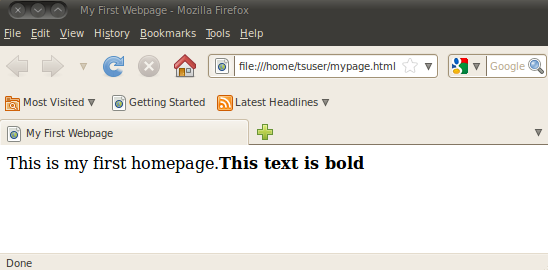
\includegraphics[scale=0.6]{First.png}

\subsubsection*{HTML Tags}
 HTML Tags are used to mark-up HTML elements.
\begin{itemize}
\item They are surrounded by the two characters $< and >$ (angle brackets).
\item Normally in pairs like $<b>$ and $</b>$ where first is start tag and the second tag is end tag.
\item The text between the start and end tags is the element content.
\item Not case sensitive\\

\underline{\textbf{Tag Attributes:}}

\item It provides additional information about the HTML elements.
\item The $<tag>$ tells the browser to do something, while the attribute tells the browser how to do it.
\item It always come in name/value pairs like this: $name="value".$
\item name is added to the start tag of an HTML element and the value is surrounded by  single or double quotes.\\
\end{itemize}

\subsubsection*{Basic HTML Tags:}
%\begin{table}[ht]
%\centering 
\begin{tabular}{| c | c | c |}\hline
\textbf{Tag Name} & \textbf{Tag} & \textbf{Description} \\\hline
 Starting Tag & $<html>$.....$</html>$ & Used to Display Webpages\\ \hline
 Body Tag & $<body>$.....$</body>$ & Body of the document\\ \hline
 & $<h1>$.....$</h1>$ & \\ 
 & $<h2>$.....$</h2>$ & Descriptive info, \\
 Heading Tag & ........  & for displaying Headings \\ 
 & ........  & in different formats \\
 &  $<h6>$......$</h6>$ &  \\ \hline
 Paragraph Tag & $<p>$.....$</p>$ & Starts and Stops the Paragraph\\ \hline
 Break Tag & $<br>$ & Used to break a line if needed\\ \hline
 Horizontal Rule Tag & $<hr>$ & Horizontal Line\\ \hline
 Comments...Tag & $<!- some text.... -->$ & To comment the required text \\ \hline
\end{tabular}
%\end{table}
\\
\subsubsection*{\texttt{<!DOCTYPE>} Declaration}
Every HTML document should start with a $<!DOCTYPE>$ declaration that tells the browser what version of HTML the document is written in. Whereas $<!DOCTYPE>$ used in current version of HTML(i.e., HTML5) is much shorter than previous version of HTML(i.e., HTML4).\\

\textbf{\underline{\small{HTML4:}}}
\begin{verbatim}
        <!DOCTYPE HTML PUBLIC "-//W3C//DTD HTML 4.01//EN" 
                         "http://www.w3.org/TR/html4/strict.dtd">
\end{verbatim}

\textbf{\underline{\small{HTML5:}}}
\begin{verbatim}
        <!DOCTYPE HTML>
\end{verbatim}

\subsubsection*{Character encoding declaration}
A charater encoding declaration is a mechanism for specifying the character encoding used to store or transmit a document.\\
The first line inside $<head>$ is the one that defines the character encoding for the document. This is another element that's been simplified.\\

\textbf{\small{\underline{HTML4:}}}
\begin{verbatim}
        <meta http-equiv="Content-Type" content="text/html; 
                                               charset=utf-8">
\end{verbatim}
HTML5 improves on this by reducing the character encoding $<meta>$ tag to the bare minimum:\\

\textbf{\small{\underline{HTML5:}}}
\begin{verbatim}
        <meta charset="utf-8">
\end{verbatim}
In nearly all cases, $utf-8$ is the value you will be using in your documents. A full explanation of character encoding is beyond the scope of this chapter, and it probably won’t be that interesting to you, either. Nonetheless, if you want to delve a little deeper,

you can go to this link \texttt{\underline{http://www.w3schools.com/html/html\_charset.asp}}

\subsubsection*{HTML Elements}
The basic structure for all HTML documents is simple and should include the following minimum elements or tags:\\

$<html>$ - The main container for HTML pages\\

$<head>$ - The container for page header information\\

$<title>$ - The title of the page\\

$<body>$ - The main body of the page\\

{\large{\textbf{Explanation:}}}\\

\underline{\textbf{The $<$html$>$ Element:}}\\

The $<html>$ element is the containing element for the whole HTML document. Each HTML document should have one $<html>$ and each document should end with a closing $</html>$ tag.\\
Following two elements appear as direct children of an $<html>$ element:
\begin{itemize}
\item $<head>$
\item $<body>$
\end{itemize}
As such, start and end HTML tags enclose all the other HTML tags you use to describe the Web page.\\

\underline{\textbf{The $<$head$>$ Element:}}\\
\begin{itemize}
\item The $<head>$ element is just a container for all other header elements.
\item It should be the first thing to appear after the opening $<html>$ tag.
\item Each $<head>$ element should contain a $<title>$ element indicating the title of the document.
\end{itemize}

\underline{\textbf{Example:}}
\begin{verbatim}
    <!DOCTYPE html>
        <html>
            <head>
                <meta charset="utf-8">
                <title> My First Webpage </title>
            </head>
        </html>
\end{verbatim}

\begin{lstlisting}
    <!DOCTYPE html>
        <html>
            <head>
                <meta charset="utf-8">
                <title> My First Webpage </title>
            </head>
        </html>
\end{lstlisting}

\underline{\textbf{The $<$title$>$ Element:}}\\

This element is a child of the $<head>$ element. It is used in several ways:
\begin{itemize}
\item It displays at the very top of a browser window.
\item It is used as the default name for a bookmark in browsers such as IE and Netscape.
\item It is used by search engines that use its content to help index pages.
\end{itemize}
Therefore it is important to use a title that really describes the content of your site. The $<title>$ element should contain only the text for the title and it may not contain any other elements.\\

\underline{\textbf{Example:}}
\begin{verbatim}
     <head>
          <title>HTML Basic tags</title>
     </head>
\end{verbatim}

\underline{\textbf{The $<$body$>$ Element:}}\\

The $<body>$ element appears after the $<head>$ element and contains the part of the Web page that you actually see in the main browser window, which is sometimes referred to as body content.\\

A $<body>$ element may contain anything from a couple of paragraphs under a heading.

\underline{\textbf{Example:}}
\begin{verbatim}
     <body>
          <p>This is a paragraph tag.</p>
     </body>
\end{verbatim}

\subsubsection*{HTML Attributes}

Attributes are another important part of HTML markup. An attribute is used to define the characteristics of an element and is placed inside the element's opening tag. \\

All attributes are made up of two parts: a name and a value:
\begin{itemize}
\item The \emph{name} is the property you want to set. 
\item The \emph{value} is what you want the value of the property to be.
\end{itemize}
The value of the attribute should be put in double quotation marks, and is separated from the name by the equals sign. \\

\underline{\textbf{Alignment:}}
\begin{itemize}
\item It is possible to align block elements (tables, images, objects, paragraphs, etc.) on the canvas with the \textbf{align} attribute$(name = align)$. 
\item Although this attribute may be set for many HTML elements, its range of possible values sometimes differs from element to element.
\item Here we only discuss the meaning of the align attribute for text
\item Possible values for the align attribute are as follows:
\end{itemize}

\underline{\textbf{Possible Values:}}\\

\begin{center}
\begin{tabular}{| c | c |}\hline
\textbf{Values} & \textbf{Description} \\ \hline
left & text lines are rendered flush left. \\ \hline
center & text lines are centered.\\ \hline
right & text lines are rendered flush right.\\ \hline
justify & text lines are justified to both margins.\\ \hline
\end{tabular}
\end{center}

\underline{\textbf{Example:}}
\begin{verbatim}
    <!DOCTYPE html>
        <html>
            <head>
                <meta charset="utf-8">
                <title>My First Webpage</title>
            </head>
            <body>
                <h1>This is a heading</h1>
                <h2 align="center">This is a heading</h2>
                <h3 align="right">This is a heading</h3>
                <h4 align="center">This is a heading</h4>
                <h5 align="left">This is a heading</h5>
                <h6 align="right">This is a heading</h6>
            </body>
        </html>
\end{verbatim}
\underline{\textbf{Output:}}\

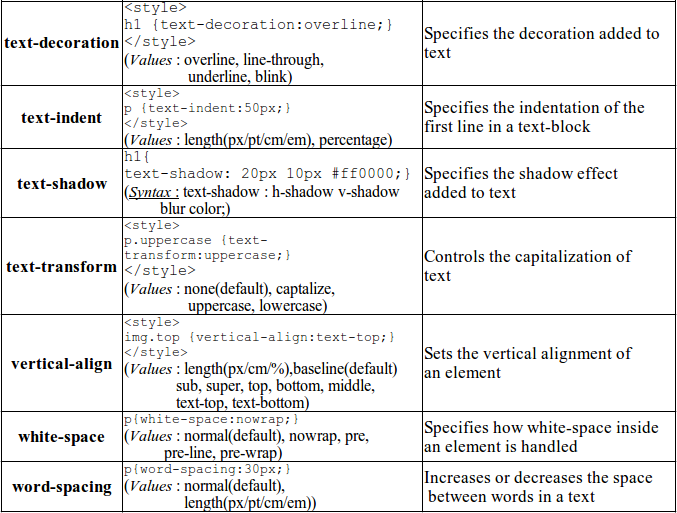
\includegraphics[height = 65mm, width = 120mm]{Second.png}

\underline{\textbf{Example:}}\\

\hspace{1cm}Creating a sample webpage by putting all tags together tags in one single document.
\begin{verbatim}
<!DOCTYPE html>
    <html>
        <head>
            <meta charset="utf-8">
            <title> My First Webpage </title>
         <body>
             <h1 align="center">My First Webpage</h1>
             <p>Welcome to my first webpage. I am writing
                this page using a text editor.<!-- These comments
                doesn't affect the web presentation -->
             </p>
             <p>By learning html, I'll be able to create webpages
                      like................<br>
                      which I am of course.
             </p>
        </body>
        </head>
    </html>
\end{verbatim}

\underline{\textbf{Output:}}\\

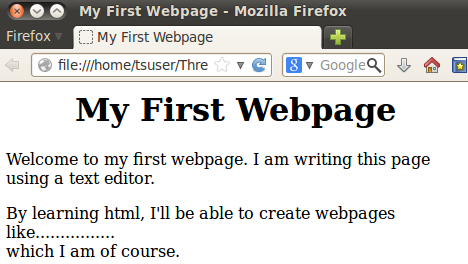
\includegraphics[height = 61mm, width = 120mm]{Three.png}

\subsubsection {Difference Between Elements and Attributes}
\begin{center}
\begin{tabular}{| c | c |}\hline
\textbf{Elements} & \textbf{Attributes} \\ \hline
represents structure & Defines a property \\ 
or semantics & for an element\\\hline
consists of a start tag, & Consists of an attribute / value pair\\
content, and an end tag & and appears within element's start tag\\ \hline
\end{tabular}
\end{center}

\underline{\textbf{Example:}}\\

$<p\ align = ``right">$ This is the content of the paragraph element.
                                                         $</p>$\\
$<p>$ $\Rightarrow$ Element\\
align\ \  $\Rightarrow$ Attribute\\
``right''\ $\Rightarrow$ Value\\

\subsection*{What’s new in HTML5}
HTML5 was created to make the coding process easier and more logical. The unique and impressive features HTML5 comes with are in the multimedia department. Many of the features it comes with have been created with the consideration that users should be able to run heavy content on low-powered devices. The syntactic features include the new $<video>$, $<audio>$ and $<canvas>$ elements, but also integration of vector graphics content (what we knew before as being the $<object>$ tags). This means that multimedia and graphic content on the web will be handled and executed easier and faster, without the need of plugins or APIs.

\subsubsection*{New Elements}

\begin{tabular}{|l|l|}\hline
\multicolumn{1}{ |c| }{\textbf{Tag}} & \multicolumn{1}{ |c| }{\textbf{Description}} \\ \hline
$<article>$  &	Defines an article in the document \\ \hline
$<aside>$ &	Defines content aside from the page content \\ \hline
$<audio>$ &     Defines sound, such as music or other audio streams.\\ \hline
$<video>$ &    Defines video, such as a movie clip or other video streams.\\ \hline
$<source>$ &    is used to specify multiple media resources for media elements,\\ & such as $<video>$ and $<audio>.$ \\ \hline
$<bdi>$ &	Defines a part of text that might be formatted in a \\ & different direction from other text outside it \\ \hline
$<details>$ & 	Defines additional details that the user can view or hide \\ \hline
$<dialog>$  & 	Defines a dialog box or window\\ \hline
$<figcaption> $  &	Defines a caption for a $<figure>$ element \\ \hline
$<figure>$  &	Defines self-contained content, like illustrations,\\ & diagrams, photos, code listings, etc. \\ \hline
$<footer>$  & 	Defines a footer for the document or a section \\ \hline
$<header>$  & 	Defines a header for the document or a section \\ \hline
$<main>$  & 	Defines the main content of a document \\ \hline
$<mark>$  & 	Defines marked or highlighted text \\ \hline
$<menuitem>$  &  	Defines a command/menu item that the user can\\ & invoke from a popup menu \\ \hline
$<meter>$  & 	Defines a scalar measurement within a known range\\ \hline
$<nav>$  & 	Defines navigation links in the document \\ \hline
$<progress>$  &	Defines the progress of a task \\ \hline
$<rp>$  &	Defines what to show in browsers that do not support\\ & ruby annotations \\ \hline
$<rt>$  & 	Defines an explanation/pronunciation of characters \\ &(for East Asian typography) \\ \hline
\end{tabular}


\begin{tabular}{|l|l|}\hline
\multicolumn{1}{ |c| }{\textbf{Tag}} & \multicolumn{1}{ |c| }{\textbf{Description}} \\ \hline

$<ruby>$  &	Defines a ruby annotation (for East Asian typography) \\ \hline
$<section>$  & 	Defines a section in the document \\ \hline
$<summary>$  & 	Defines a visible heading for a $<details>$ element \\ \hline
$<time>$  &	Defines a date/time \\ \hline
$<wbr>$  & 	Defines a possible line-break \\ \hline
\end{tabular}
%==============================================================================================================================
%==============================================================================================================================
\section*{Basic Tags in HTML}
\subsection*{Formatting Tags}
The HTML tags are used to format the appearance of the text on your web page. This can jazz up the look of the web page, however, too much variety in the text formatting can also look displeasing.\

Some of the text formatting tags are as follows:\
\begin{description}
\item[Bold Text] $<b>.......</b>$

\hspace{1cm}The text in between the tags will be bold, and stand out against text around it, the same as in a word processor.\

\underline{\textbf{Example:}}

\hspace{1cm} $<p>$The following word uses a $<b>$bold$</b>$ typeface.$</p>$

\underline{\textbf{Result:}}

\hspace{1cm} The following word uses a \textbf{bold} typeface.\

\item[Italic Text] $<i>.......</i>$

\hspace{1cm} Also working the same way as a word processor, italics displays the text at a slight angle.\

\underline{\textbf{Example:}}

\hspace{1cm}$<p>$The following word uses a $<i>$italicized$</i>$ typeface.$</p>$

\underline{\textbf{Result:}}

\hspace{1cm} The following word uses a \textit{italicized} typeface.\

\item[Underline Text] $<u>......</u>$

\hspace{1cm} Again, the same as underline in a word processor. Note that html links are already underlined and don't need the extra tag. Also $<ins>$ tag is also used similar to this.\

\underline{\textbf{Example:}}

\hspace{1cm}$<p>$The following word uses a $<u>$underlined$</u>$ typeface.$</p>$

\underline{\textbf{Result:}}

\hspace{1cm} The following word uses a \underline{underlined} typeface.\

\item[Strike-out Text] $<strike>......</strike>$

\hspace{1cm}Puts a line right through the centre of the text, crossing it out. Often used to show that text is old and no longer relevant. Also works by using $<s>...... </s>$ instead. Also to delete text $<del>$ works as same.\

\underline{\textbf{Example:}}

\hspace{1cm}$<p>$The following word uses a $<strike>$ strikethrough $</strike>$ typeface.$</p>$

\underline{\textbf{Result:}}

\hspace{1cm}The following word uses a \st{strikethrough} typeface.\

\item[Preformatted Text] $<pre>......</pre>$

\hspace{1cm} Any text between the pre tags, including spaces, carriage returns and punctuation, will appear in the browser as it would in a text editor (normally browsers ignore multiple spaces)\

\underline{\textbf{Example:}}

\hspace{2cm}$<pre>$\

\hspace{3cm}function testFunction( strText )\{\

\hspace{3.8cm} alert (strText);\

\hspace{3cm}\}\

\hspace{2cm}$</pre>$

\underline{\textbf{Result:}}
\begin{verbatim}
           function testFunction( strText ){
                alert (strText)
           }
\end{verbatim}

\item[Emphasis] $<em>.....</em>$

\hspace{1cm}Used to emphasize text, which usually appears in italics, but can vary according to your browser.\

\underline{\textbf{Example:}}

\hspace{1cm}$<p>$The following word uses a $<em>$emphasis$</em>$ typeface.$</p>$

\underline{\textbf{Result:}}

\hspace{1cm}The following word uses a \emph{emphasis} typeface.\

\item[Strong Emphasis] $<strong>.....</strong>$

\hspace{1cm}Used to emphasize text more, which usually appears in bold, but can vary according to your browser.\

\underline{\textbf{Example:}}

\hspace{1cm}$<p>$The following word uses a $<strong>$strong emphasis$</strong>$ typeface.$</p>$

\underline{\textbf{Result:}}

\hspace{1cm}The following word uses a \textbf{strong emphasis} typeface.\

\item[Smaller Text] $<small>......</small>$

\hspace{1cm}The content of the $<small>$ element is displayed one font size smaller than the rest of the text surrounding it.\

\underline{\textbf{Example:}}

\hspace{1cm}$<p>$The following word uses a $<small>$small$</small>$ typeface.$</p>$

\underline{\textbf{Result:}}

\hspace{1cm}The following word uses a \small{small} typeface.\

\item[Larger Text] $<big>.....</big>$

\hspace{1cm} The content of the $<big>$ element is displayed one font size larger than the rest of the text surrounding it.\

\underline{\textbf{Example:}}

\hspace{1cm}$<p>$The following word uses a $<big>$big$</big>$ typeface.$</p>$
This will produce following result:

\underline{\textbf{Result:}}

\hspace{1cm}The following word uses a {\large{big}} typeface.\


\item[Superscript Text]$<sup>.....</sup>$

\hspace{1cm} The content of a $<sup>$ element is written in superscript; the font size used is the same size as the characters surrounding it but is displayed half a characters height above the other characters.\

\underline{\textbf{Example:}}

\hspace{1cm}$<p>$The following word uses a $<sup>$superscript$</sup>$ typeface.$</p>$

\underline{\textbf{Result:}}

\hspace{1cm}The following word uses a $^{superscript}$ typeface.\

\item[Subscript Text] $<sub>.....</sub>$

\hspace{1cm}The content of a $<sub>$ element is written in subscript; the font size used is the same as the characters surrounding it, but is displayed half a characters height beneath the other characters.\

\underline{\textbf{Example:}}

\hspace{1cm}$<p>$The following word uses a $<sub>$subscript$</sub>$ typeface.$</p>$

\underline{\textbf{Result:}}

\hspace{1cm}The following word uses a $_{subscript}$ typeface.
\end{description}

\begin{center}
\begin{tabular}{| c | c | c |}\hline
\textbf{Tags} & \textbf{Description} & \textbf{Formatted Text} \\ \hline
$<b>$ & Bold Text & \textbf{bold} \\ \hline
$<i>$ & Italic Text & \textit{italicized}\\ \hline
$<u>$ & Underline Text & \underline{underlined} \\ \hline
$<strike>$ & Strike-out Text & \st{strikethrough}\\ \hline
%$<pre>$ & Preformatted Text &\\ \hline
$<em>$ & Emphasis & \emph{emphasis}\\ \hline
$<strong>$ & Strong Emphasis & \textbf{strong emphasis}\\ \hline
$<small>$ & Smaller Text & \small{small}\\ \hline
$<large>$ & Larger Text & {\large{large}}\\ \hline
$<sup>$ & Superscript & $25^{th} Aug$\\ \hline
$<sub>$ & Subscript & $H_{2}O$\\ \hline
\end{tabular}
\end{center}

\underline{\textbf{Example:}}

\hspace{1cm}Simple example of HTML document using formatted tags.
\begin{verbatim}
    <!DOCTYPE HTML>
        <html>
            <body>
                <p><b>This text is bold</b></p>
                <p><strong>This text is strong</strong></p>
                <p><i>This text is italic</i></p>
                <p><em>This text is emphasized</em></p>
                <p><u>This is computer output</u></p>
                <p>This is<sub> subscript</sub>
                         and <sup>superscript</sup></p>
            </body>
        </html>
\end{verbatim}

\underline{\textbf{Output:}}\

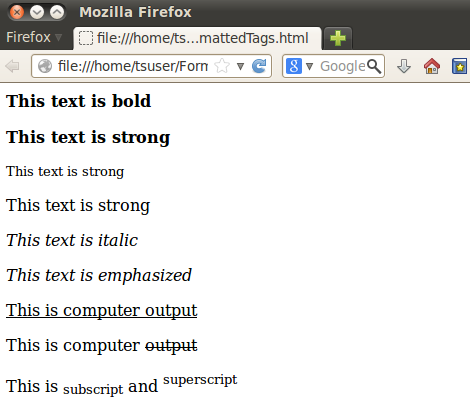
\includegraphics[height = 61mm, width = 120mm]{FormattedText.png}

\section*{HTML Fonts}
Font face and color depends entirely on the computer and browser that is being used to view your page. But the $<font>$ tag is used to add style, size, and color to the text on your site.\

The font tag is having three attributes called size, color, and face to customize your fonts.\

To change any of the font attributes at any time within your page, simply use the $<font>$ tag. The text that follows will remain changed until you close with the $</font>$ tag. You can change any or all of the font attributes at the one time, by including all the required changes within the one $<font>$ tag.\

\begin{center}
\begin{tabular}{| c | c | c |}\hline
\textbf{Attribute} & \textbf{Value} & \textbf{Description} \\ \hline
Size & number & Specifies the size of text \\ \hline
face & font\_family & Specifies the font of text \\ \hline
color & rgb(x,x,x)\#xxxxxx colorname & Specifies the color of text\\ \hline
\end{tabular}
\end{center}
\subsubsection*{Attributes}
\begin{description}
\item[Font Size]\
 
You can set the size of your font with size attribute. The range of accepted values is from 1(smallest) to 7(largest). The default size of a font is 3.\

\underline{\textbf{Example:}}
\begin{verbatim}
    <!DOCTYPE HTML>
        <html>
            <head>
                <title>My Webpage</title>
            </head>
            <body>
                <font size="1">Font size="1"</font></br>
                <font size="2">Font size="2"</font></br>
                <font size="3">Font size="3"</font></br>
                <font size="4">Font size="4"</font></br>
                <font size="5">Font size="5"</font></br>
                <font size="6">Font size="6"</font></br>
                <font size="7">Font size="7"</font>
            </body>
        </html>
\end{verbatim}

\underline{\textbf{Output:}} \\
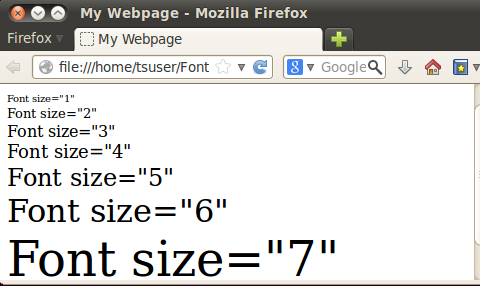
\includegraphics[height = 61mm, width = 120mm]{FontSize.png}\

\item[Font Face]\

You can set any font you like using face attribute but be aware that if the user viewing the page doesn't have the font installed, they will not be able to see it. Instead they will default to Times New Roman of your font with size attribute. See below few examples on using different font face.\

\underline{\textbf{Example:}}
\begin{verbatim}
<!DOCTYPE HTML>
    <html>
        <head>
            <title>My Webpage</title>
        </head>
        <body>
            <font face="Times New Roman" size="5">
                Times New Roman
            </font></br>
            <font face="Verdana" size="5">
                Verdana
            </font></br>
            <font face="Comic sans MS" size="5">
                Comic Sans MS
            </font></br>
            <font face="WildWest" size="5">
                WildWest</font></br>
            <font face="Bedrock" size="5">
                Bedrock
            </font>
        </body>
    </html>
\end{verbatim}

\underline{\textbf{Output:}}\

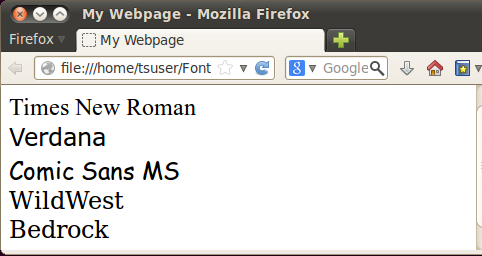
\includegraphics[height = 61mm, width = 120mm]{FontFace.png}\ 


\item[Font Color]\

You can set any font color you like using color attribute. You can specify the color that you want by either the color name or hexadecimal code for that color. Check a complete list of HTML Color Name with Codes.\

\underline{\textbf{Example:}}
\begin{verbatim}
<!Doctype HTML>
    <html>
        <head>
            <title>My Webpage</title>
        </head>
        <body>
            <font color="#FF00FF">
                This text is hexcolor #FF00FF
            </font><br />
            <font color="red">
                This text is red
            </font>
        </body>
    </html>
\end{verbatim}

\underline{\textbf{Output:}}\\

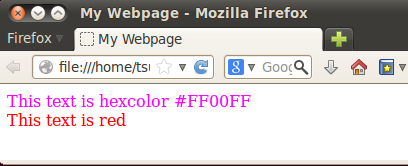
\includegraphics[height = 35mm, width = 100mm]{FontColor.png}\

\item[bgcolor Attribute]\
\begin{itemize}
\item The bgcolor attribute specifies the background color of a document.
\item It is an attribute for $<body>$
\end{itemize}

\textbf{Syntax:}\

$<body\  bgcolor="color\_name|hex\_number|rgb\_number">$\

\textbf{Attributes Values}\

Table showing attribute values:
\begin{center}
\begin{tabular}{| c | c |}\hline
\textbf{Value} & \textbf{Description} \\ \hline
color\_name & Specifies the background color with a color name (like "red") \\ \hline
hex\_number & Specifies the background color with a hex code (like "\#ff0000") \\ \hline
rgb\_number & Specifies the background color with an rgb code (like "rgb(255,0,0)") \\ \hline
\end{tabular}
\end{center}

\underline{\textbf{Example:}}
\begin{verbatim}
 <!DOCTYPE HTML>
     <html>
         <head>
             <title>My Webpage</title>
         </head>
         <body bgcolor="#DEB887">
             <h1 align="center">
                 My First Webpage 
             </h1>
             <p>
                 Welcome to my first colorful webpage.
                 I am writing this page using a text editor
                 and used background color.
                 <!-- These comments doesn't affect the web
                                           presentation -->
             </p>
             <p>
                 By learning html, I'll be able to create webpages 
                     like................<br>
                     which I am of course.
             </p>
         </body>
     </html>
\end{verbatim}  

\underline{\textbf{Output:}}\

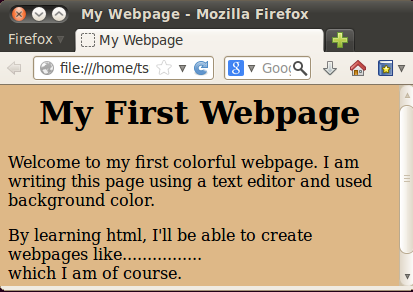
\includegraphics[height = 80mm, width = 120mm]{Bgcolor.png}\

\item[Header Tag] $<header>$
\begin{itemize}
\item $< header >$ tag specifies a header for a document or section.
\item used as a container for introductory content or set of navigational links.
\item multiple $< header >$ elements are allowed\\
\end{itemize}

\item[Footer Tag] $<footer>$ 
\begin{itemize}
\item $<footer>$ tag defines a footer for a document or section.
\item contains the author of the document, copyright information, links to terms of use, contact information...
\item multiple $<footer>$ elements are allowed
\end{itemize}
\end{description}

\subsection*{Lists}
\hspace{1cm} HTML lists appear in web browsers as bulleted lines of text. There are actually three different types of HTML lists,They are as follows,
\begin{enumerate}
\item Unordered lists (bullets)
\item Ordered lists (numbers)
\item Definition lists (think: dictionaries).
\end{enumerate}
 Each list type utilizes its own unique list tag, which we'll demonstrate below.\
\begin{description}
\item[Unordered lists]\

An unordered list ($<ul>$) signifies to a web browser that all list items contained inside the $<ul>$ and$<\backslash ul>$ tag should be rendered with a bullet preceding the text. The default bullet type for most web browsers is a full disc (black circle), but this can be adjusted using an HTML attribute called \emph{"type"}.\

\textbf{Default Bullet List:}
\begin{verbatim}
    <!DOCTYPE HTML>
        <html>
            <head>
                <title>My Webpage</title>
            </head>
            <body>
                <h4 align="center">Shopping List</h4>
                <ul>
                    <li>Milk</li>
                    <li>Toilet Paper</li>
                    <li>Cereal</li>
                    <li>Bread</li>
                </ul>
            </body>
        </html>
\end{verbatim}

\underline{\textbf{Output:}}\

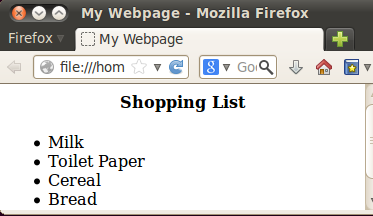
\includegraphics[scale=0.7]{DefaultList.png}\

To render a list with a different bullet type, add a type attribute to the unordered list element. Using the same code in the example above, replace the $<ul>$ line from the previous example with any of the lines listed below to change the bullet from disc shape to another shape.\

\textbf{Values for \emph{type} attributes:}\

$<$ul type = "square"$>$ -  A square hollow bullet

$<$ul type = "disc"$>$ - A solid bullet (the default)

$<$ul type = "circle"$>$ - A hollow bullet\

\underline{\textbf{Example:}} $<$ul type = "square"$>$
\begin{verbatim}
    <!DOCTYPE HTML>
        <html>
            <head>
                <title>My Webpage</title>
            </head>
            <body>
                <h4 align = "center">List of Subjects</h4>
                <ul type = "square">
                    <li>Hindi</li>
                    <li>English</li>
                    <li>Maths</li>
                    <li>Physics</li>
                </ul>
            </body>
        </html>
\end{verbatim}

\underline{\textbf{Output:}}

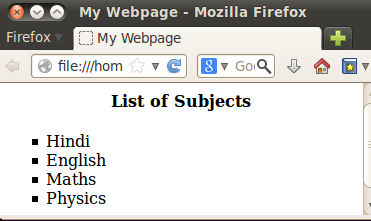
\includegraphics[scale=0.7]{square.png}\

\underline{\textbf{Example:}} $<$ul type = "disc"$>$
\begin{verbatim}
    <!DOCTYPE HTML>
        <html>
            <head>
                <title>My Webpage</title>
            </head>
            <body>
                <h4 align = "center">List of Subjects</h4>
                <ul type = "disc">
                    <li>Hindi</li>
                    <li>English</li>
                    <li>Maths</li>
                    <li>Physics</li>
                </ul>
            </body>
        </html>
\end{verbatim}


\underline{\textbf{Output:}}

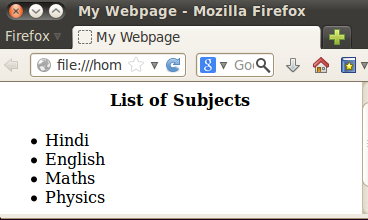
\includegraphics[scale=0.6]{Disc.png}\

\underline{\textbf{Example:}} $<$ul type = "circle"$>$
\begin{verbatim}
    <!DOCTYPE HTML>
        <html>
            <head>
                <title>My Webpage</title>
            </head>
            <body>
                <h4 align = "center">List of Subjects</h4>
                <ul type = "circle">
                    <li>Hindi</li>
                    <li>English</li>
                    <li>Maths</li>
                    <li>Physics</li>
                </ul>
            </body>
        </html>
\end{verbatim}

\underline{\textbf{Output:}}\

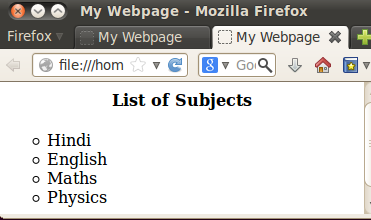
\includegraphics[scale=0.7]{circle.png}\

\item[Ordered lists]\

An ordered list is defined using the $<ol>$ tag, and list items placed inside of an ordered list are preceded with numbers instead of bullets.

The numbering of an HTML list can be changed to letters or Roman Numerals by once again adjusting the \emph{type} attribute.\

\textbf{Default Number List:}
\begin{verbatim}
    <!DOCTYPE HTML>
        <html>
            <head>
                <title>My Webpage</title>
            </head>
            <body>
                <h4 align="center">Shopping List</h4>
                <ol>
                    <li>Milk</li>
                    <li>Toilet Paper</li>
                    <li>Cereal</li>
                    <li>Bread</li>
                </ol>
            </body>
        </html>
\end{verbatim}
\underline{\textbf{Output:}}\\

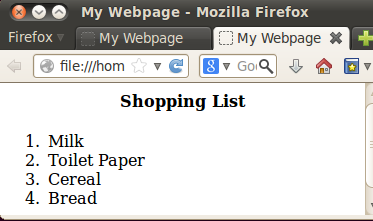
\includegraphics[scale=0.8]{NumberList.png}\



\textbf{Values of \emph{type} Attribute:}\

$<$ol type="I"$>$ - Upper-Case Numerals.

$<$ol type="i"$>$ - Lower-Case Numerals.

$<$ol type="a"$>$ - Lower-Case Letters.

$<$ol type="A"$>$ - Upper-Case Letters.\

\underline{\textbf{Example:}} $<$ol type = "I"$>$
\begin{verbatim}
    <!DOCTYPE HTML>
        <html>
            <head>
                <title>My Webpage</title>
            </head>
            <body>
                <h4 align = "center">List of Subjects</h4>
                <ol type = "I">
                    <li>Hindi</li>
                    <li>English</li>
                    <li>Maths</li>
                    <li>Physics</li>
                </ol>
            </body>
        </html>
\end{verbatim}

\underline{\textbf{Output:}}\

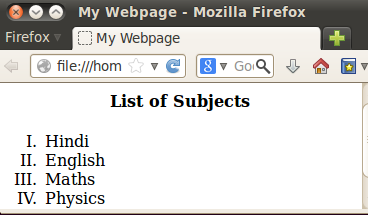
\includegraphics[scale=0.7]{OL1.png}\

\underline{\textbf{Example:}} $<$ol type = "i"$>$
\begin{verbatim}
    <!DOCTYPE HTML>
        <html>
            <head>
                <title>My Webpage</title>
            </head>
            <body>
                <h4 align = "center">List of Subjects</h4>
                <ol type = "i">
                    <li>Hindi</li>
                    <li>English</li>
                    <li>Maths</li>
                    <li>Physics</li>
                </ol>
            </body>
        </html>
\end{verbatim}

\underline{\textbf{Output:}}\

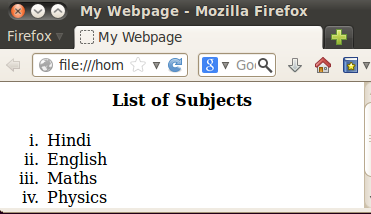
\includegraphics[scale=0.7]{OL2.png}\

\underline{\textbf{Example:}} $<$ol type = "a"$>$
\begin{verbatim}
    <!DOCTYPE HTML>
        <html>
            <head>
                <title>My Webpage</title>
            </head>
            <body>
                <h4 align = "center">List of Subjects</h4>
                <ol type = "a">
                    <li>Hindi</li>
                    <li>English</li>
                    <li>Maths</li>
                    <li>Physics</li>
                </ol>
            </body>
        </html>
\end{verbatim}

\underline{\textbf{Output:}}\

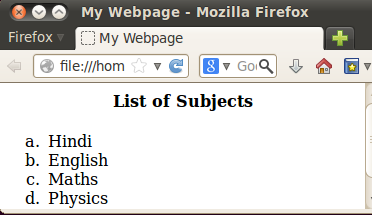
\includegraphics[scale=0.7]{OL3.png}\

\underline{\textbf{Example:}} $<$ol type = "A"$>$
\begin{verbatim}
    <!DOCTYPE HTML>
        <html>
            <head>
                <title>My Webpage</title>
            </head>
            <body>
                <h4 align = "center">List of Subjects</h4>
                <ol type = "A">
                    <li>Hindi</li>
                    <li>English</li>
                    <li>Maths</li>
                    <li>Physics</li>
                </ol>
            </body>
        </html>
\end{verbatim}

\underline{\textbf{Output:}}

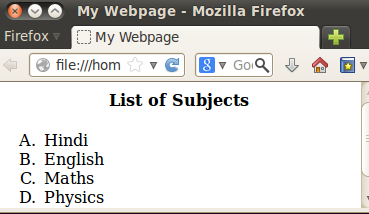
\includegraphics[scale=0.56]{OL4.png}\


The \emph{start} attribute allows you to further customize an HTML ordered list by setting a new starting digit for the ordered list element.

\underline{\textbf{Example:}}
\begin{verbatim}
    <!DOCTYPE HTML>
        <html>
            <head>
                <title>My Webpage</title>
            </head>
            <body>
                <h4 align = "center">List of Subjects</h4>
                <ol start = "5">
                    <li>Hindi</li>
                    <li>English</li>
                    <li>Maths</li>
                    <li>Physics</li>
                </ol>
            </body>
        </html>
\end{verbatim}

\underline{\textbf{Output:}}\

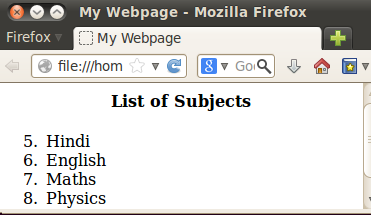
\includegraphics[scale=0.7]{Start.png}\\

\item[Definition term lists]\

HTML definition lists ($<dl>$) are list elements that have a unique array of tags and elements; the resulting listings are similar to those you'd see in a dictionary.These lists are important because they provide a context for the text with which they are associated.\

$<dl>$ - opening clause that defines the start of the list\

$<dt>$ - list item that defines the definition term\

$<dd>$ - definition of the list item\
\begin{description}
\item[DL] $<dl>$\

A definition list is the container element for DT($<dt>$) and DD($<dd>$) elements. The DL($<dl>$ element should be used when you want incorporate a definition of a term in your document, it is often used in glossaries to define many terms, it is also used in “normal” documents when the author wishes to explain a term in a more detail (Like this definition).\

\item[DT] $<dt>$\

The term currently being defined in the definition list. This element contains inline data.\

\item[DD] $<dd>$\

The definition description element contains data that describes a definition term. This data may be either inline, or it may be block level.\

These lists displace the word term ($<dt>$) in such a way that it rests just above the definition element ($<dd>$) to offer a very unique look. For best, results we suggest bolding the definition terms with the bold tag $<b>$.

\underline{\textbf{Example:}}
\begin{verbatim}
<!DOCTYPE HTML>
    <html>
        <head>
            <title>My Webpage</title>
        </head>
        <body>
            <p>Definition List items </p>
            <dl>
                <dt>
                    <b>
                        HTML
                    </b>
                </dt>
                    <dd>
                        This stands for
                        Hyper Text Markup Language
                    </dd>
                <dt>
                    <b>
                        HTTP
                    </b>
                </dt>
                    <dd>
                        This stands for
                        Hyper Text Transfer Protocol
                    </dd>
            </dl>
        </body>      
        </html>
\end{verbatim}

\underline{\textbf{Output:}}\

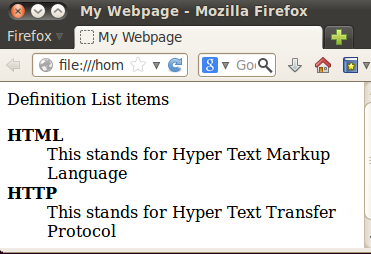
\includegraphics[scale=0.7]{Definition.png}\
\end{description}
\end{description}

\subsection*{Appropriate List Usage}


Following are just a suggestion and there is no hard and fast rule to use them:\

\textbf{Use Unordered lists for:}
\begin{itemize}
\item Link collections.
\item Short, nonsequenced groups of text.
\item Emphasizing the high points of a presentation.
\end{itemize}

\textbf{Use Ordered lists for:}
\begin{itemize}
\item Tables of contents.
\item Sets of sequential sections of text.
\item Assigning numbers to short phrases that can be referenced elsewhere.
\end{itemize}


\textbf{Use Definition lists for:}
\begin{itemize}
\item Glossaries.
\item Custom bullets - make the item after the $<dt>$ tag an icon-sized bullet image).
\item Any list of name/value pairs.
\end{itemize}
%&&&&&&&&&&&&&&&&&&&&&&&&&&&&&&&&&&&&&&&&&&&&&&&&&&&&&&&&&&&&&&&&&&&&&&&&&&&&&&&&&&&&&&&&&&&&&&&&&&&&&&&&&&&&&&&&&&&&&&&&
%&&&&&&&&&&&&&&&&&&&&&&&&&&&&&&&&&&&&&&&&&&&&&&&&&&&&&&&&&&&&&&&&&&&&&&&&&&&&&&&&&&&&&&&&&&&&&&&&&&&&&&&&&&&&&&&&&&&&&&&&
\subsection*{Links}
\hspace{1cm} Web pages can contain links that take you directly to other pages and even specific parts of a given page. These links are known as hyperlinks.\

\subsubsection*{Hyperlinks}

It allow visitors to navigate between Web sites by clicking on words, phrases, and images. Thus you can create hyperlinks using text or images available on your any web page.\

From this you will learn how to create text links between the different pages of your site, links within pages of your sites, and how to link to other sites ( or external sites).\

\textbf{URL}

\hspace{1cm}Every document on the Web has a unique address. This address is known as \underline{\textbf{U}}niform \underline{\textbf{R}}esource \underline{\textbf{L}}ocator (URL).\

\textbf{URL Elements}

\hspace{1cm} A URL is made of up several parts, each of which offers information to the Web browser to help find the page you are after. It is easier to learn the parts of a URL if you look at the most common ones first. If you look at the example URL given below, there are three key parts: the scheme, the host address, and the file path. The following sections discuss each of these in turn.\

\underline{\textbf{Example:}}\

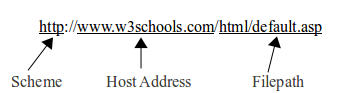
\includegraphics[scale=0.8]{URL.png}

\begin{description}
\item[The Scheme]\
The scheme identifies the type of protocol and URL you are linking to and therefore how the resource should be retrieved. For example, most Web pages use something called the \emph{Hypertext Transfer Protocol (HTTP)} to pass information to you which is why most Web pages start with \emph{http://}.

There are other schemes available and you can use based on your requirement:\

\item[Description:]\

\item[http://]\
Hypertext Transfer Protocol (HTTP) is used to request pages from Web servers and send them back from Web servers to browsers.\

\item[https://]\
Secure Hypertext Transfer Protocol (HTTPS) encrypts the data sent between the browser and the Web server using a digital certificate.\

\item[ftp://]\
File Transfer Protocol is another method for transferring files on the Web. While HTTP is a lot more popular for viewing Web sites because of its integration with browsers, FTP is still commonly used protocol to transfer large files across the Web and to upload source files to your Web server.\

\item[file://]\
Used to indicate that a file is on the local hard disk or a shared directory on a LAN.\
\end{description}

\textbf{The Host Address}\

The host address is where a Web site can be found, either the IP address (four sets of numbers between 0 and 258, for example 68.178.157.132 ) or more commonly the domain name for a site such as \emph{www.tutorialspoint.com}. Note that \emph{"www"} is not actually part of the domain name although it is often used in the host address.it has nothing to do with the protocol used.\

\textbf{The Filepath}\\

The filepath always begins with a forward slash character, and may consist of one or more directory or folder names. Each directory name is separated by forward slash characters and the filepath may end with a filename at the end. Here \emph{index.htm} is the filename which is available in html directory.\

\subsection*{Linking Documents}

\textbf{ The $<a>$ Element:}\

A link is specified using the $<a>$ element. This element is called anchor tag as well. Anything between the opening $<a>$ tag and the closing $<\backslash a>$ tag becomes part of the link and a user can click that part to reach to the linked document.\

\textbf{Syntax:}\

$<a\ href="Document URL" attr\_name="attr\_value"...more\ attributes />$\

\textbf{Anchor Attributes:}\

Following are most frequently used attributes for $<a>$ tag.
\begin{itemize}
\item \textbf{href:} Specifies the URL of the target of a hyperlink. Its value is any valid document URL, absolute or relative, including a fragment identifier or a JavaScript code fragment.
\item \textbf{target:} Specify where to display the contents of a selected hyperlink. If set to "\_blank" then a new window will be opened to display the loaded page, if set to "\_top" or "\_parent" then same window will be used to display the loaded document, if set to "\_self" then loads the new page in current window. By default its "\_self".
\item \textbf{name \& id:} Attributes places a label within a document. When that label is used in a link to that document, it is the equivalent of telling the browser to goto that label.
\item \textbf{event:} Attributes like onClick, onMouseOver etc. are used to trigger any Javascript ot VBscript code.
\item \textbf{title:} Attribute lets you specify a title for the document to which you are linking. The value of the attribute is any string, enclosed in quotation marks. The browser might use it when displaying the link, perhaps flashing the title when the mouse passes over the link.
\item \textbf{accesskey:} Attribute attribute provides a keyboard shortcut that can be used to activate a link.\

For example, you could make the T key an access key so that when the user presses either the Alt or Ctrl key on his keyboard (depending on his operating system) along with the T key, the link gets activated.\
\end{itemize}
\underline{\textbf{Example:}}
\begin{verbatim}
     <html>
          <head>
               <title>My Webpage</title>
          </head>
          <body>
               <a href="http://www.google.com/" target="_blank" >
                                                Google Home Page</a></br>
               <a href="http://www.gmail.com/" target="_self" >
                                                Gmail Login Page</a></br>
               <a href="http://www.change-images.com/" target="_top" >       
                                               Change Images Home</a>
          </body>
     </html>
\end{verbatim}
\underline{\textbf{Output:}}\

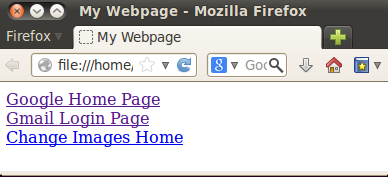
\includegraphics[scale=0.9]{TextLinks.png}

As now we know that how to create hyper text link using text and how to use images in your web page. Now we will learn how to use images to create hyper links. \

\underline{\textbf{Example:}}
\begin{verbatim}
     <html>
          <head>
               <title>Webpage Using images</title>
          </head>
          <body>
               <a href="http://www.google.com/index.htm"  
                                               target="_self" ></br>
                   <img src="/images/home.gif" alt="Google Home Page"     
                                                      border="0"/>
               </a>
          </body>
     </html>
\end{verbatim}

This will create following hyperlink at google.com home.\


\underline{\textbf{Output:}}\

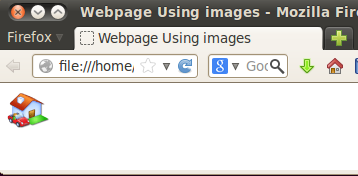
\includegraphics[scale=0.9]{ImageLink.png}

%&&&&&&&&&&&&&&&&&&&&&&&&&&&&&&&&&&&&&&&&&&&&&&&&&&&&&&&&&&&&&&&&&&&&&&&&&&&&&&&&&&&&&&&&&&&&&&&&&&&&&&&&&&&&&&&&&&&&&&&&
%&&&&&&&&&&&&&&&&&&&&&&&&&&&&&&&&&&&&&&&&&&&&&&&&&&&&&&&&&&&&&&&&&&&&&&&&&&&&&&&&&&&&&&&&&&&&&&&&&&&&&&&&&&&&&&&&&&&&&&&&

%\chapter*{Session 2 - HTML Negivations and Tables} 
The HTML table model allows authors to arrange data -- text, preformatted text, images, links, forms, form fields, other tables, etc. -- into rows and columns of cells.
\subsection*{A simple table}
Here is a trivial table of two rows and two columns:
\begin{verbatim}
    <table border="1">
        <tr>
            <td>Row 1, Column 1</td>
            <td>Row 1, Column 2</td>
        </tr>
        <tr>
            <td>Row 2, Column 1</td>
            <td>Row 2, Column 2</td>
        </tr>
    </table>
\end{verbatim}
\underline{\textbf{Output:}} 

%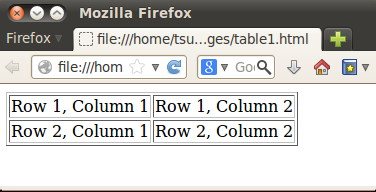
\includegraphics[height = 60mm, width = 200mm]{Table1.png}
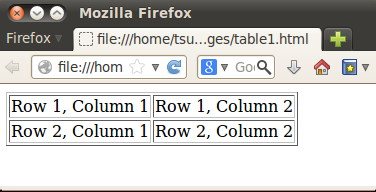
\includegraphics[scale=0.7]{Table1.png}
\begin{itemize}
\item The entire table is contained between $<table>$ and $</table>$ tags.
\item Each table row starts with a $<tr>$ tag.
\item Each cell starts with a $<td>$ tag.
\end{itemize}

\subsection*{Table Heading}
To add the column heading to the columns in the table, place the heading in $<th>$ and $</th>$ tags.
\subsection*{Captioning a table}
To add a title to a table, place the caption text between $<caption>$ and $</caption>$ tags just after the
$<table>$ tag.\\	

You can use an \emph{align = "bottom"} attribute in the $<caption>$ tag to position the caption below the table. The default placement is at the top.\\
\begin{verbatim}
    <caption align = "bottom"> Salary Details </caption>
\end{verbatim}
\underline{\textbf{Example:}}
\begin{verbatim}
    <table border = "1">
        <caption> Salary Details </caption>
        <tr> 
            <th> Name </th>
            <th> Salary </th>
        </tr>
        <tr>
            <td> Ramesh Raman </td>
            <td>5000</td>
         </tr>
         <tr>
             <td> Shabbir Hussein </td>
             <td> 7000</td>
          </tr>
    </table>
\end{verbatim}


\underline{\textbf{Output:}}

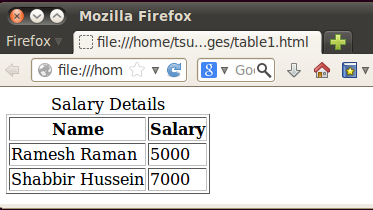
\includegraphics[height = 60mm, width = 100mm]{Table2.png}
\section*{Attributes of the $<table>$ tag}
The $<table>$ tag allows a number of optional attributes that specify the properties of the entire table.

\begin{itemize}
\item \textbf{$<$table align = "left"$>$} positions the table at the left side of the viewer window, \emph{align = "center"} centers it, and \emph{align = "right"} places it on the right side.
\item The \textbf{$<$table width = "dimension"$>$} attribute sets the width of the entire table, it is discussed above in the section on dimensions.
\item  The \textbf{$<$table border = "dimension"$>$} tells the browser to draw a border around the entire table. 
The dimension is optional and specifies how thick to make the border. \\
For example: \emph{$<table border = "5px">$}\\
specifies a five-pixel border around the table.
\end{itemize}
\subsection*{Aligning Text in Cells}
\subsubsection*{Horizontal alignment of text in cells}
Used to Justify the text in the cells, by default it justifies to left.\\
Any cell can include an align="align-type" attribute to tell the browser how to position the item in that cell.\\


The align-type can be any of:
\begin{itemize}
\item  \textbf{$<$td align = "left"$>$} to left-justify the contents of the cell.
\item \textbf{$<$td align = "center"$>$} to center the contents of the cell.
\item \textbf{$<$td align = "right"$>$} to right-justify the contents of the cell.
\item \textbf{$<$td align = "justify"$>$} to to justify the text; that is, if the item is a text string too long to fit on one line, all the lines but the last will be stretched to form straight left and right margins.
\item You can use $<td align = "char">$ for columns of numbers with decimals so that they are aligned on the decimal point.
\end{itemize}
\subsubsection*{Vertical alignment for a whole row}
Used specify where the items are placed vertically in their cells by using a valign attribute in the $<tr>$ tag for that row. \

The valign attribute can take these values:
\begin{itemize}
\item \textbf{$<$tr valign = "top"$>$} says to put each item at the top of its cell.
\item \textbf{$<$tr valign = "middle"$>$} says to center each item vertically within its cell.
\item \textbf{$<$tr valign = "bottom"$>$} says to put each item at the bottom of its cell.
\end{itemize}
\underline{\textbf{Example:}}\\
\begin{verbatim}
    <table border = "1">
        <caption> Salary Details </caption>
        <tr>
            <th> Name </th>
            <th> Salary </th>
        </tr>
        <tr align = "center">  
            <td align = "right"> Ramesh Raman </td>
            <td align = "center">5000</td>
        </tr>
        <tr align = "center">
            <td align = "right"> Shabbir Hussein </td>
            <td align = "center"> 7000</td>
        </tr>
    </table>
\end{verbatim}
\textbf{Output:}\\
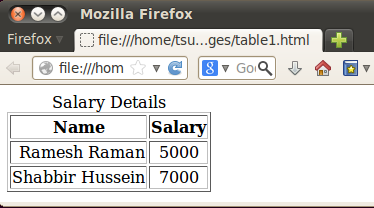
\includegraphics[height = 60mm, width = 100mm]{Table3.png}
\subsubsection*{Alignment for an entire column}
It is difficult to add an align = "..." attribute in each cell of a column. A better way is use a group
of \textbf{$<$col$>$} tags before the first row of the table, each of these tags specifies the alignment for that whole column.\\

\underline{\textbf{Example:}}
\begin{verbatim}
     <table border =  "1">
        <caption>Numbers</caption>
        <col align = "left" width = "50">
        <col align = "right" width = "50">
        <tr>
            <td> I </td>
            <td> One</td> 
        </tr>
        <tr>
            <td> II </td>
            <td> Two</td> 
        </tr>
        <tr>
            <td> III </td>
            <td> Three</td> 
        </tr>
    </table>
\end{verbatim}

\underline{\textbf{Output:}}

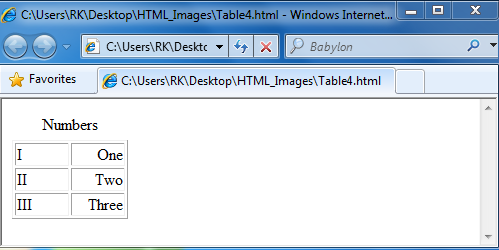
\includegraphics[height = 60mm, width = 100mm]{Table4.png}

The first $<col>$ tag says that the first column's cells will be left-justified. The second $<col>$ tag says to right-justify the cells of the second column.

\subsubsection*{Column grouping}
If you have groups of columns with the same attribute values, you can use a $<colgroup>$ tag before each group of $<col>$ tags to specify attributes for that group.
\begin{verbatim}
    <table>
        <colgroup align = "center">
            <col width = "3pi">
            <col width = "5pi" span = "4">
        <colgroup align = "right">
            <col width = "4pi">
            <col width = "8pi">
             ...
    </table>
\end{verbatim}
The example above defines seven columns. The first five are all centered and the next two are right-justified.

\subsubsection*{Cellpadding and Cellspacing}
There are two attribiutes called cellpadding and cellspacing which you will use to adjust the white space in your table cell. Cellspacing defines the width of the border, while cellpadding represents the distance between cell borders and the content within.\\

\underline{\textbf{Example:}}\\

\begin{verbatim}
    <table border = "1" cellpadding = "15" cellspacing = "5">
        <tr>
            <th>Name</th>
            <th>Salary</th>
        </tr>
        <tr>
            <td>Ramesh Raman</td>
            <td>5000</td>
        </tr>
        <tr>
            <td>Shabbir Hussein</td>
            <td>7000</td>
        </tr>
    </table>
\end{verbatim}
\underline{\textbf{Output:}}

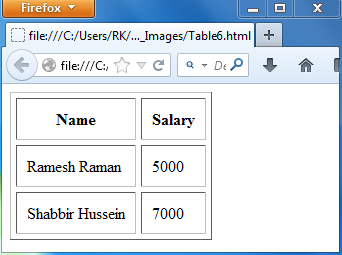
\includegraphics[height = 60mm, width = 100mm]{Table5.png}

\subsubsection*{Colspan and Rowspan Attributes}
Colspan attribute is used to merge two or more columns into a single column and rowspan attribute is used to merge two or more rows. 
\begin{verbatim}
    <table border = "1">
        <tr>
            <th>Column 1</th>
            <th>Column 2</th>
            <th>Column 3</th>
        </tr>
        <tr>
            <td rowspan = "2">Row 1 Cell 1</td>
            <td>Row 1 Cell 2</td>
            <td>Row 1 Cell 3</td>
        </tr>
        <tr>
            <td>Row 2 Cell 2</td>
            <td>Row 2 Cell 3</td>
        </tr>
        <tr>
            <td colspan = "3">Row 3 Cell 1</td>
        </tr>
    </table>
\end{verbatim}
\underline{\textbf{Output:}}\\
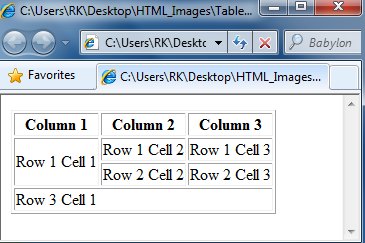
\includegraphics[height = 60mm, width = 100mm]{Table6.png}

\subsubsection*{Tables Backgrounds}
You can set table background using of the following two ways:
\begin{itemize}
\item \textbf{bgcolor attribute} - You can set background color for whole table or just for one cell.
\item \textbf{background attribute} - You can set background image for whole table or just for one cell.
\end{itemize}
\emph{NOTE : You can set border color also using bordercolor attribute.}\\

\underline{\textbf{Example:}}
\begin{verbatim}
    <table border = "5" bordercolor = "green" bgcolor = "gray">
        <tr>
            <th>Column 1</th>
            <th>Column 2</th>
            <th>Column 3</th>
        </tr>
        <tr>
            <td rowspan = "2">Row 1 Cell 1</td>
            <td bgcolor = "red">Row 1 Cell 2</td>
            <td>Row 1 Cell 3</td>
        </tr>
        <tr>
            <td>Row 2 Cell 2</td>
            <td>Row 2 Cell 3</td>
        </tr>
        <tr>
            <td colspan = "3">Row 3 Cell 1</td>
        </tr>
    </table>
\end{verbatim}
\textbf{Output:}\\
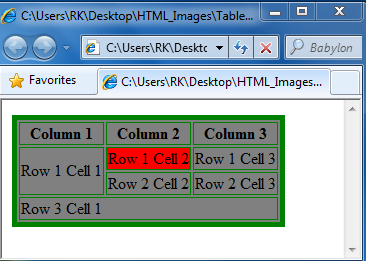
\includegraphics[height = 60mm, width = 100mm]{Table7.png}

\subsection*{Using a Header, Body, and Footer}
Tables can be divided into three portions a header, a body, and a foot. \\
The head and foot are rather similar to headers and footers in a word-processed document that remain the same for every page, while the body is the main content of the table.

The three elements for separating the head, body, and foot of a table are:
\begin{itemize}
\item \textbf{$<$thead$>$} - to create a separate table header.
\item \textbf{$<$tbody$>$} - to indicate the main body of the table.
\item \textbf{$<$tfoot$>$} - to create a separate table footer.
\end{itemize}
A table may contain several $<tbody>$ elements to indicate different pages or groups of data. But it is notable that $<thead>$ and $<tfoot>$ tags should appear before $<tbody>$
\begin{verbatim}
    <table border = "1" width = "100%">
        <thead>
            <tr>
                <td colspan = "4">This is the head of the table</td>
            </tr>
        </thead>
        <tfoot>
            <tr>
                <td colspan = "4">This is the foot of the table</td>
            </tr>
        </tfoot>
        <tbody>
            <tr>
                <td>Cell 1</td>
                <td>Cell 2</td>
                <td>Cell 3</td>
                <td>Cell 4</td>
            </tr>
            <tr>
                 ...more rows here containing four cells...
            </tr>
        </tbody>
        <tbody>
            <tr>
                <td>Cell 1</td>
                <td>Cell 2</td>
                <td>Cell 3</td>
                <td>Cell 4</td>
            </tr>
            <tr>
                  ...more rows here containing four cells...
            </tr>
        </tbody>
    </table>
\end{verbatim}


\underline{\textbf{Output:}}\\
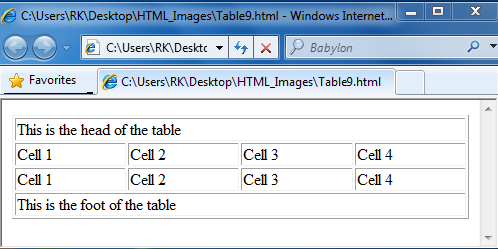
\includegraphics[height = 60mm, width = 100mm]{Table8.png}
\end{document}
